\chapter{Обзор подходов к компиляции гетерогенных приложений}\label{ch:overview}

\section{Логическое и физическое представление гетерогенных систем}\label{sec:overview/logical}

\subsection{Логическая модель API для GPGPU}\label{subsec:overview/logical/api}

При работе с графическими API для вычислений (такими как OpenCL, SYCL, Cuda и прочие), программисту приходится иметь дело с несколькими уровнями памяти.
Базовое разделение это \textbf{память хоста} -- память хостовой машины, обычно это что-то вроде обычной RAM и \textbf{память устройства}, устроенная гораздо сложнее.

В простом случае память устройства бывает следующих видов:

\begin{itemize}
\item \textbf{Глобальная} -- память на устройстве обычно большого объёма и доступная каждому EU.
\item \textbf{Виртуальная разделяемая} -- участки памяти непосредственно отображаемые на память хоста.
\item \textbf{Константная} -- память, изменение которой в программах выполняемых на устройстве запрещено.
\item \textbf{Локальная} -- память доступная только потокам внутри рабочей группы.
\item \textbf{Приватная} -- память (обычно очень небольшое её количество) доступная только конкретному EU.
\end{itemize}

Обычно тип памяти напрямую запрашивается при работе с API как на листинге~\cref{lst:oclapi}.

\begin{ListingEnv}[!h]
    \captiondelim{ } 
    \caption{Пример запроса глобального буффера в OpenCL API}\label{lst:oclapi}
    \begin{lstlisting}[language={[ISO]C++}]
  cl_context Context;
  cl_mem Buf;
  cl_int Err;
  Context = clCreateContextFromType(NULL, CL_DEVICE_TYPE_GPU, NULL, 
                                    NULL, &Err);
  // .....
  Buf = clCreateBuffer(Context, CL_MEM_READ_WRITE, BUFSZ * sizeof(int), 
                       NULL, &Err);
    \end{lstlisting}
\end{ListingEnv}

В некоторых случаях компилятор может оптимизировать работу с памятью, например сделав stateless to stateful преобразование и тогда этот буфер окажется в stateful памяти (при соблюдении ряда условий). Но программист всегда оперирует с логической моделью, так как это единственный способ написать общий код для нескольких устройтв гибридной системы.

\begin{figure}[ht]
    \centerfloat{
        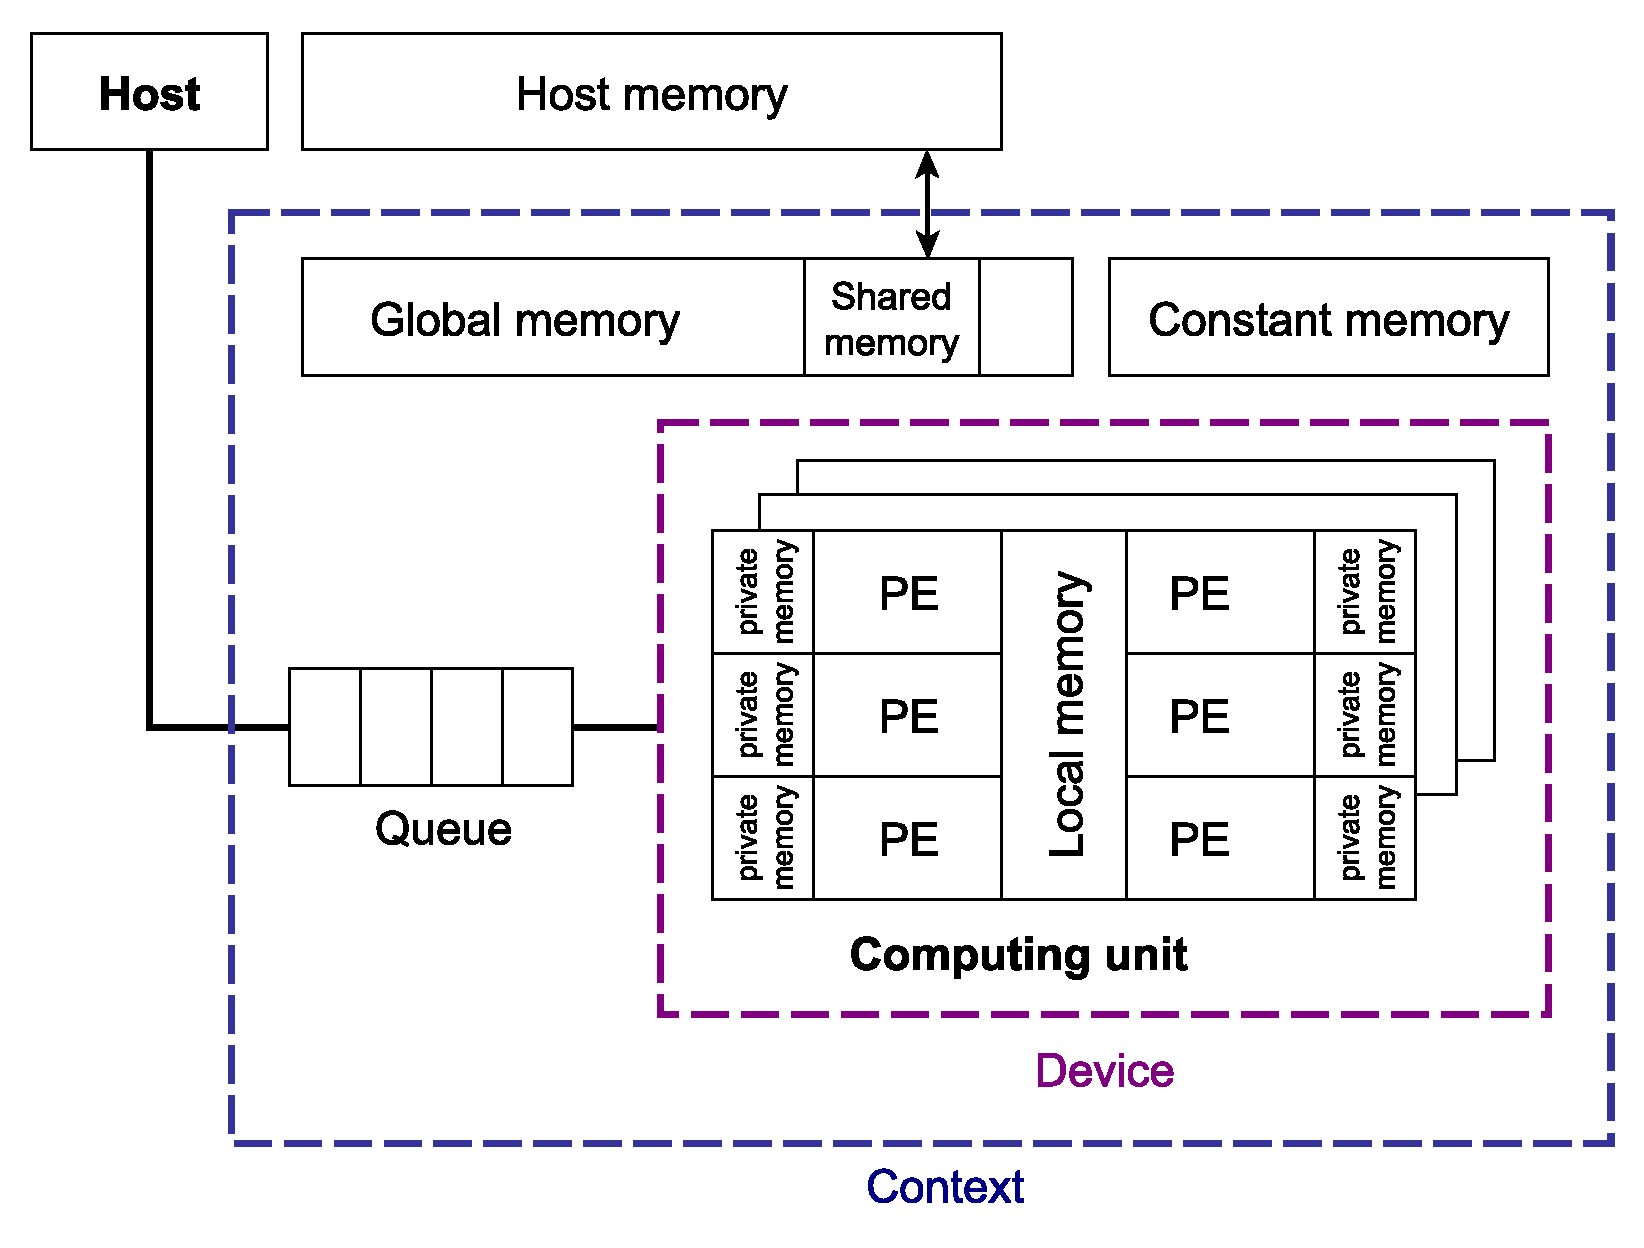
\includegraphics[scale=0.6]{Vladimirov/images/logical-memory.pdf}
    }
    \caption{Логическая модель памяти}\label{fig:logical-memory}
\end{figure}

Логическая модель памяти, характерная для таких API, как OpenCL и SYCL, представлена на рисунке~\cref{fig:logical-memory}. Ключевым понятием является computing unit (CU), это элемент кооперативной многозадачности внутри GPU. Все исполнительные устройства в пределах CU обладают доступом к общему пространству -- локальной памяти. Это небольшая и быстрая общая память. Она очень важна в таком виде. Но ещё важнее, что итерационное пространство рабочей группы позволяет потокам ждать друг друга на так называемых барьерах.

Допустим у нас есть гнездо циклов с внутренним параллелизмом, представленное на листинге~\cref{lst:nobarrier}.

\begin{ListingEnv}[!h]
    \captiondelim{ } 
    \caption{Гнездо циклов с внутренним параллелизмом}\label{lst:nobarrier}
    \begin{lstlisting}[language={[ISO]C++}]
for (auto i : Ni)
  for (auto j : Nj)
    parallel for (auto k : Nk)
      do(i, j, k);
    \end{lstlisting}
\end{ListingEnv}

Это довольно плохой случай, так как мы можем распараллелить только самый вложенный цикл и получается, что мы должны постоянно входить в параллельное исполнение и выходить из него. Но если порядок по k не важен, и $N_k$ не велико, то мы можем воспользоваться барьерами рабочей группы. Тогда это гнездо циклов трансформируется в следующий более выгодный вид, приведённый на листинге~\cref{lst:localbarrier}.

\begin{ListingEnv}[!h]
    \captiondelim{ } 
    \caption{Гнездо циклов с барьером внутри}\label{lst:localbarrier}
    \begin{lstlisting}[language={[ISO]C++}]
parallel for (auto k : Nk)
  for (auto i : Ni)
    for (auto j : Nj) {
       do(i, j, k);
       barrier(k);
    }
    \end{lstlisting}
\end{ListingEnv}

Разница в том что теперь для каждого элемента параллелизма оба дорогих вложенных цикла исполняются на своём исполнительном устройстве. Это на некоторых бенчамрках, таких как битоническая сортировка позволяют выиграть до тридцати процентов производительности и более даже в простом скалярном случае.

\subsection{Физическая модель памяти}\label{subsec:overview/logical/physmem}

На физическом уровне память устройства делится на обладающую и не обладающую состоянием.

Обладающая состоянием (stateful) память это такая память где каждый буфер имеет точку привязки (binding point) и есть поддержка в железе для быстрого преобразования binding table index (BTI) и смещения в буфере в физический адрес. У каждой адресации массива есть незримое состояние: для каждого индекса BTI есть реальный физический адрес куда отображена память и размер буфера по этому адресу, а иногда и нечто другое. Работа со stateful памятью за счёт аппаратной поддержки может быть очень эффективна, но фактически сырые (то есть stateless) указатели в такой модели оказываются запрещены: они позволяют слишком много.

Разумеется когда появляется необходимость отображать память с хостовой машины, где никаких точек привязки уже нет, а, напротив, есть такие вещи как указатели и даже динамические структуры, состоящие из указателей


\begin{figure}[ht]
    \centerfloat{
        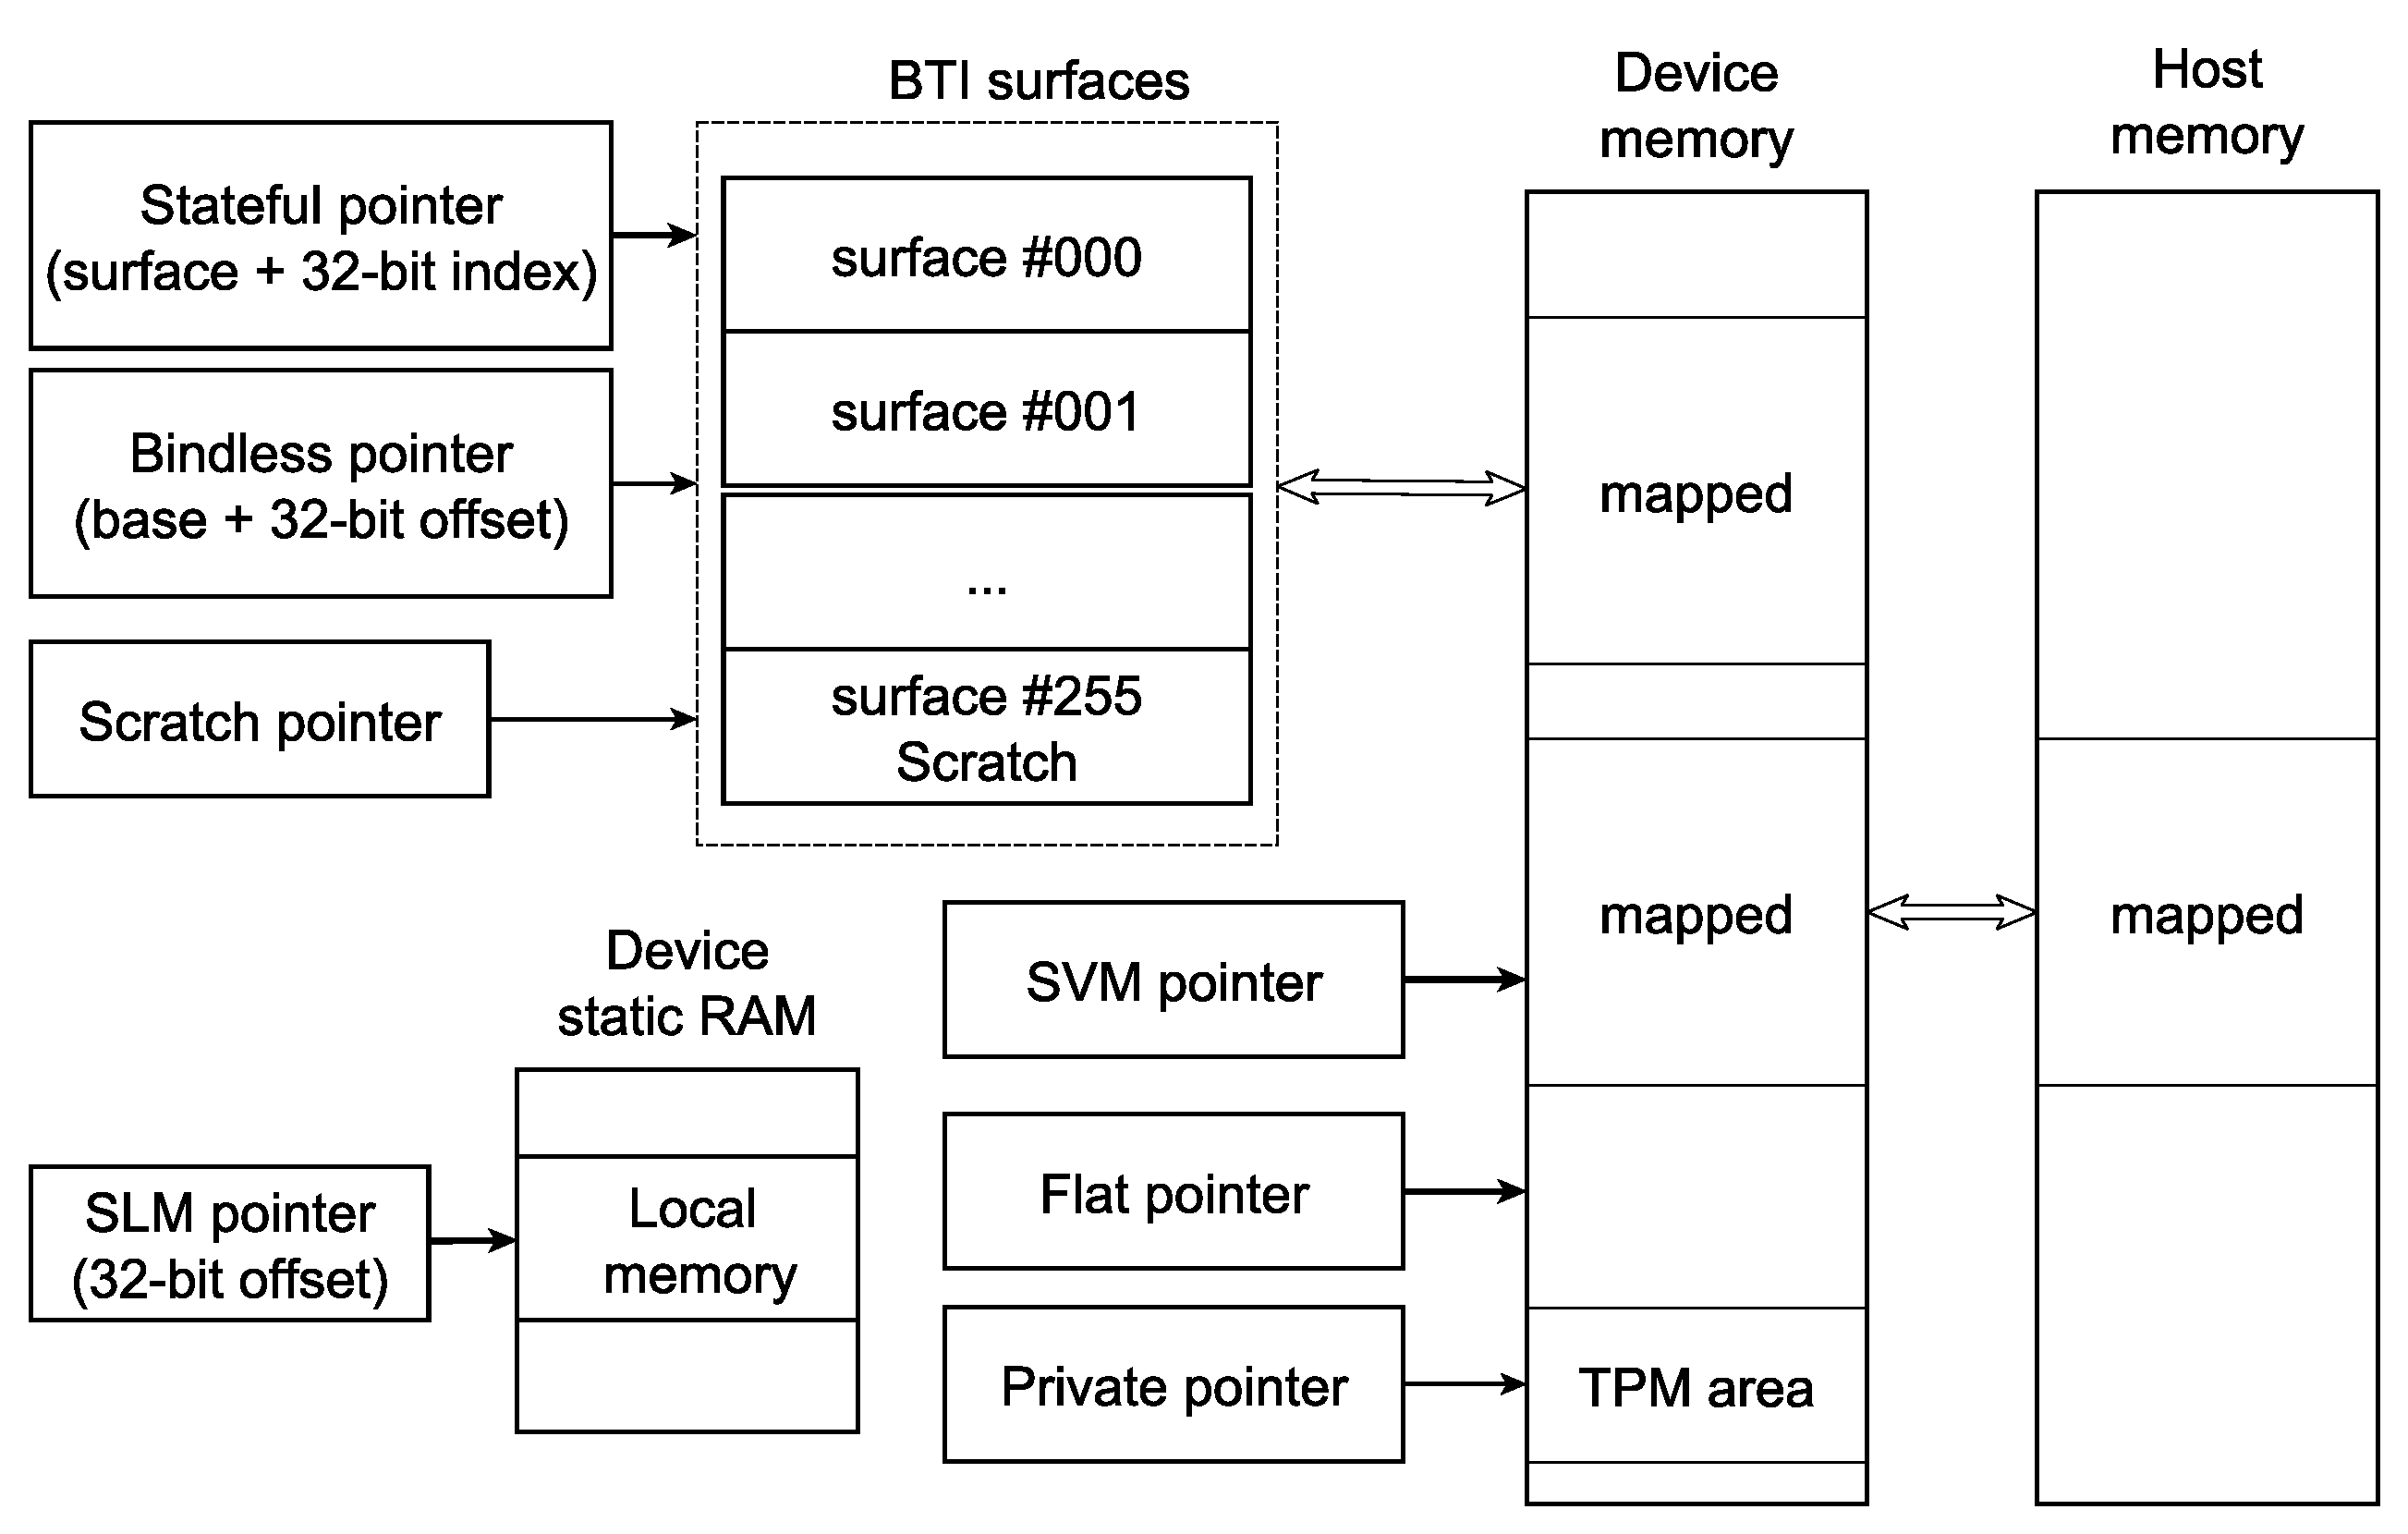
\includegraphics[scale=0.5]{Vladimirov/images/memory-scheme.pdf}
    }
    \caption{Схема физической памяти}\label{fig:memory-scheme}
\end{figure}

На рисунке~\ref{fig:memory-scheme} изображена реалистичная схема физической памяти.

TODO: тут что-то описать про физическую память, показать листинги и прочее.

\subsection{Векторный характер графических систем команд}\label{subsec:overview/logical/hw}

Все гетерогенные вычисления нужны в основном затем, чтобы максимизировать производительность.
Для этих целей в средней видеокарточке используемой в гетерогенных системах обычно просто нет операционной системы -- её драйвер это драйвер операционной системы хоста.
В связи с эти для таких устройств (это верно и для GPU и для NPU) характерно.

\begin{enumerate}
\item Отсутствие накладных расходов на переключение контекста (нет OS).
\item Сравнительно далёкая и дорогая глобальная память.
\item Часто отсутствие кешей и короткий конвейер.
\end{enumerate}

Всё это мотивирует большие регистровые файлы.

\begin{figure}[ht]
    \centerfloat{
        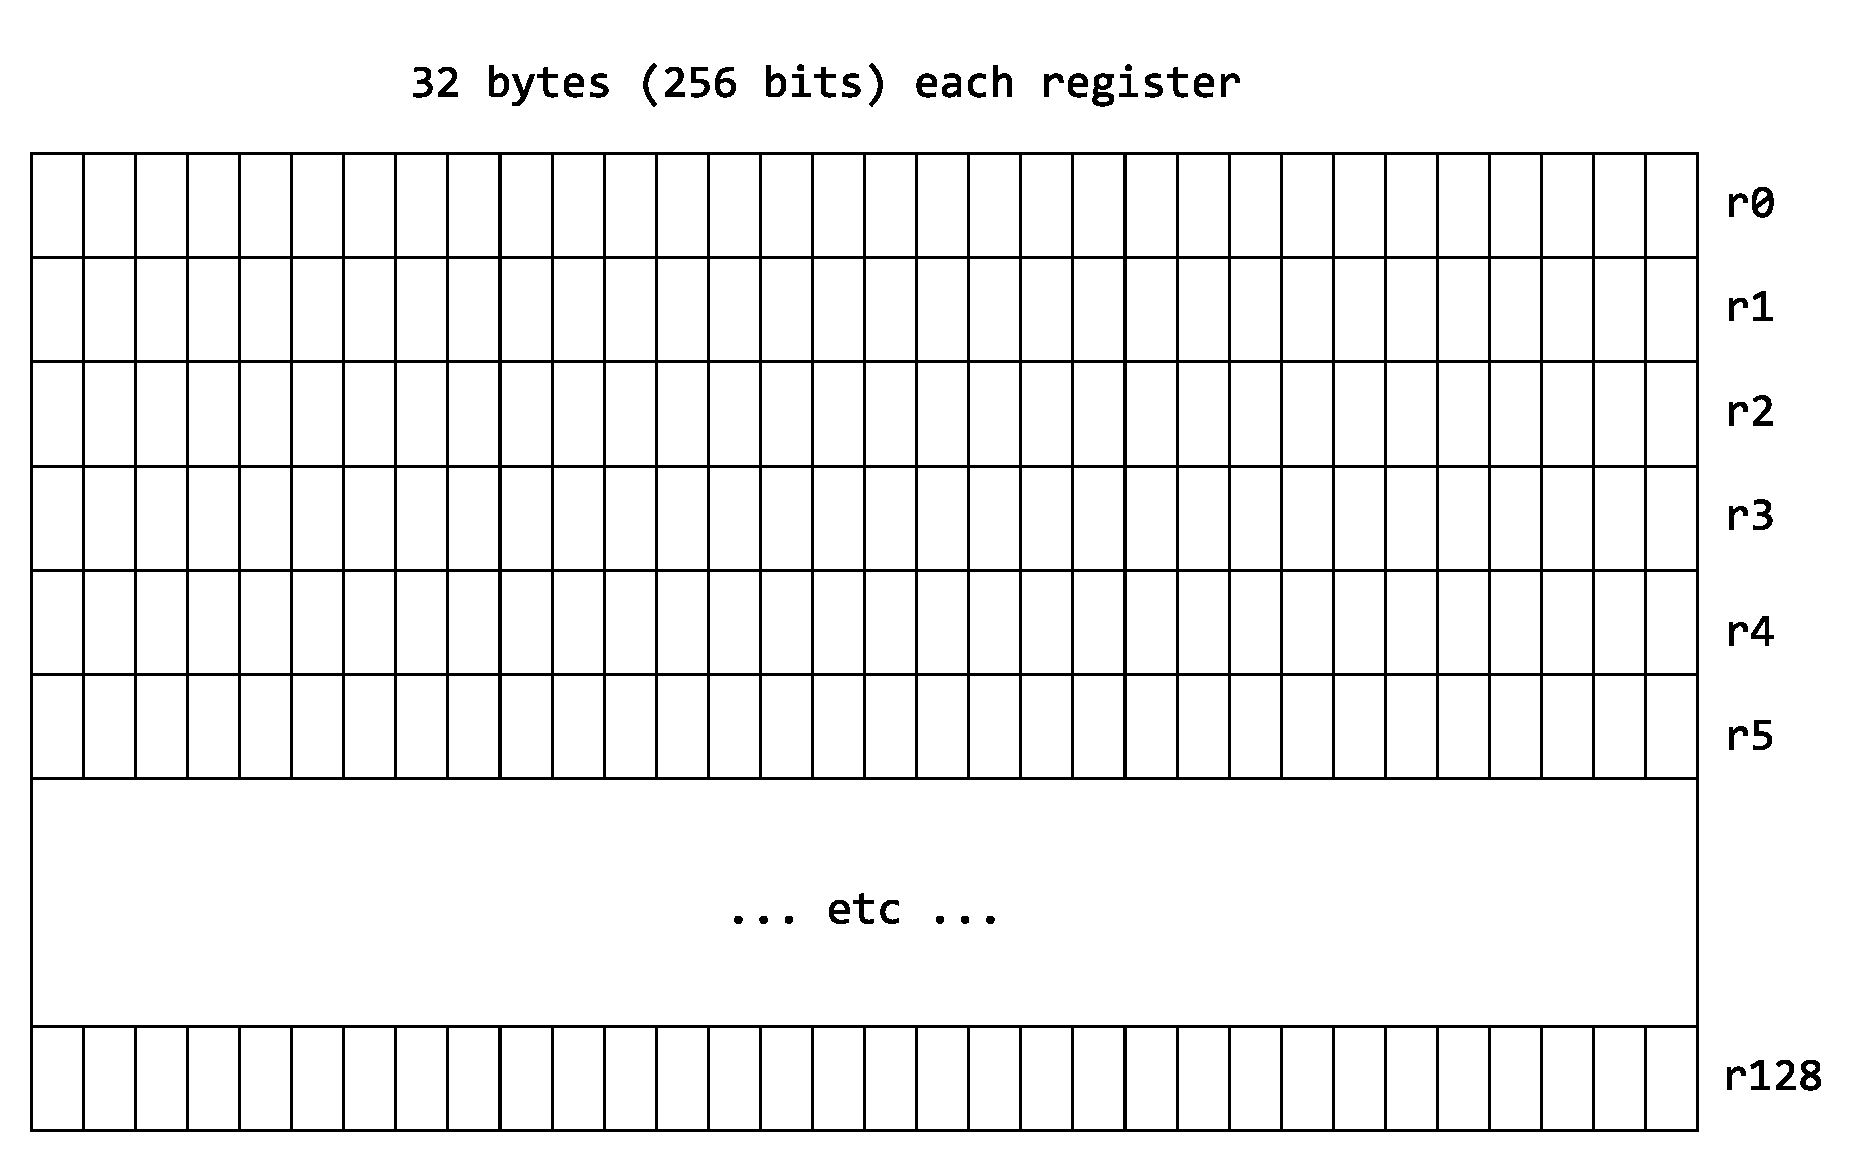
\includegraphics[scale=0.6]{Vladimirov/images/genisa-addressing-base.pdf}
    }
    \caption{Схема регистрового файла}\label{fig:genisa-addressing-base}
\end{figure}

Схема регистрового файла представлена на рисунке~\cref{fig:genisa-addressing-base}

Вовсе не всегда работа с большими регистровыми файлами удобна.

\subsection{Векторный поток управления}\label{subsec:overview/logical/simdcf}

В графических ускорителях многих производителей есть возможность использовать векторный поток управления без сведения его к скалярному случаю. В архитектуре Intel Xe это реализовано через две команды: \texttt{goto} и \texttt{join}. Особенностью команды \texttt{goto} является возможность ее предикатирования. В этом случае исполнение программы произойдет так, что для предикатированных элементов вектора произойдет переход по указанной метке, а для всех остальных элементов произойдет переход на следующую инструкцию. Команда \texttt{join} восстанавливает поток управления.

В аппаратуре подобная модель исполнения реализуется с помощью маски исполнения (\textit{англ. execution mask}). Каждый бит этой маски соответствует элементу вектора. Если бит установлен в 0, то для соответствующего элемента вычисления не производятся, если же бит установлен в 1, то для соответствующего элемента исполнение происходит в обычном режиме. В самом начале программы маска состоит из единиц. Изменения в маске производят инструкции \texttt{goto} и \texttt{join}. Команда \texttt{goto} устанавливает в соответствии с предикатом биты маски в 0, выключая линии вектора, для которых условие не выполняется. Команда \texttt{join} восстанавливает маску до того состояния, в котором она находилась до изменения соответствующим \texttt{goto}.

\begin{ListingEnv}[!h]
    \captiondelim{ } 
    \caption{Пример векторного потока управления}\label{lst:simdcf}
    \begin{verbatim}
  ...
  (W)     cmp  (8|M0)  (gt)f0.0  null<1>:d  r2.0<8;8,1>:d -1:w
  (~f0.0) goto (8|M0)            BB_3
  BB_1:
  (W)     add  (8|M0)            r3.0<1>:d  r2.0<8;8,1>:d  1:w
  (f0.0)  goto (8|M0)            BB_5
  BB_2:
          join (8|M0)            BB_3
  BB_3:
          add  (8|M0)            r3.0<1>:d  r2.0<8;8,1>:d -1:w
  BB_4:
          join (8|M0)            BB_5
  BB_5:
  ...
    \end{verbatim}
\end{ListingEnv}

На листинге~\cref{lst:oclapi}. пример кода c векторным потоком управления на языке ассемблера для архитектуры графических ускорителей Intel. В данном примере реализовано проверка того, что в регистре r.2.0 лежит значение большее, чем -1, а результат сравнения записан во флаговый регистр f0.0. Далее следует предикатированный регистром f0.0 условный переход: если условие для данной линии исполнения выполняется, то не происходит переход в базовый блок BB\_3, и к данным элементам прибавляется 1, а результат записывается в регистр r3.0. Для других элементов следует переход в базовый блок BB\_3, где из остальных элементов вычитается 1, а результат так же записывается в регистр r3.0.

\begin{figure}[ht]
    \centerfloat{
        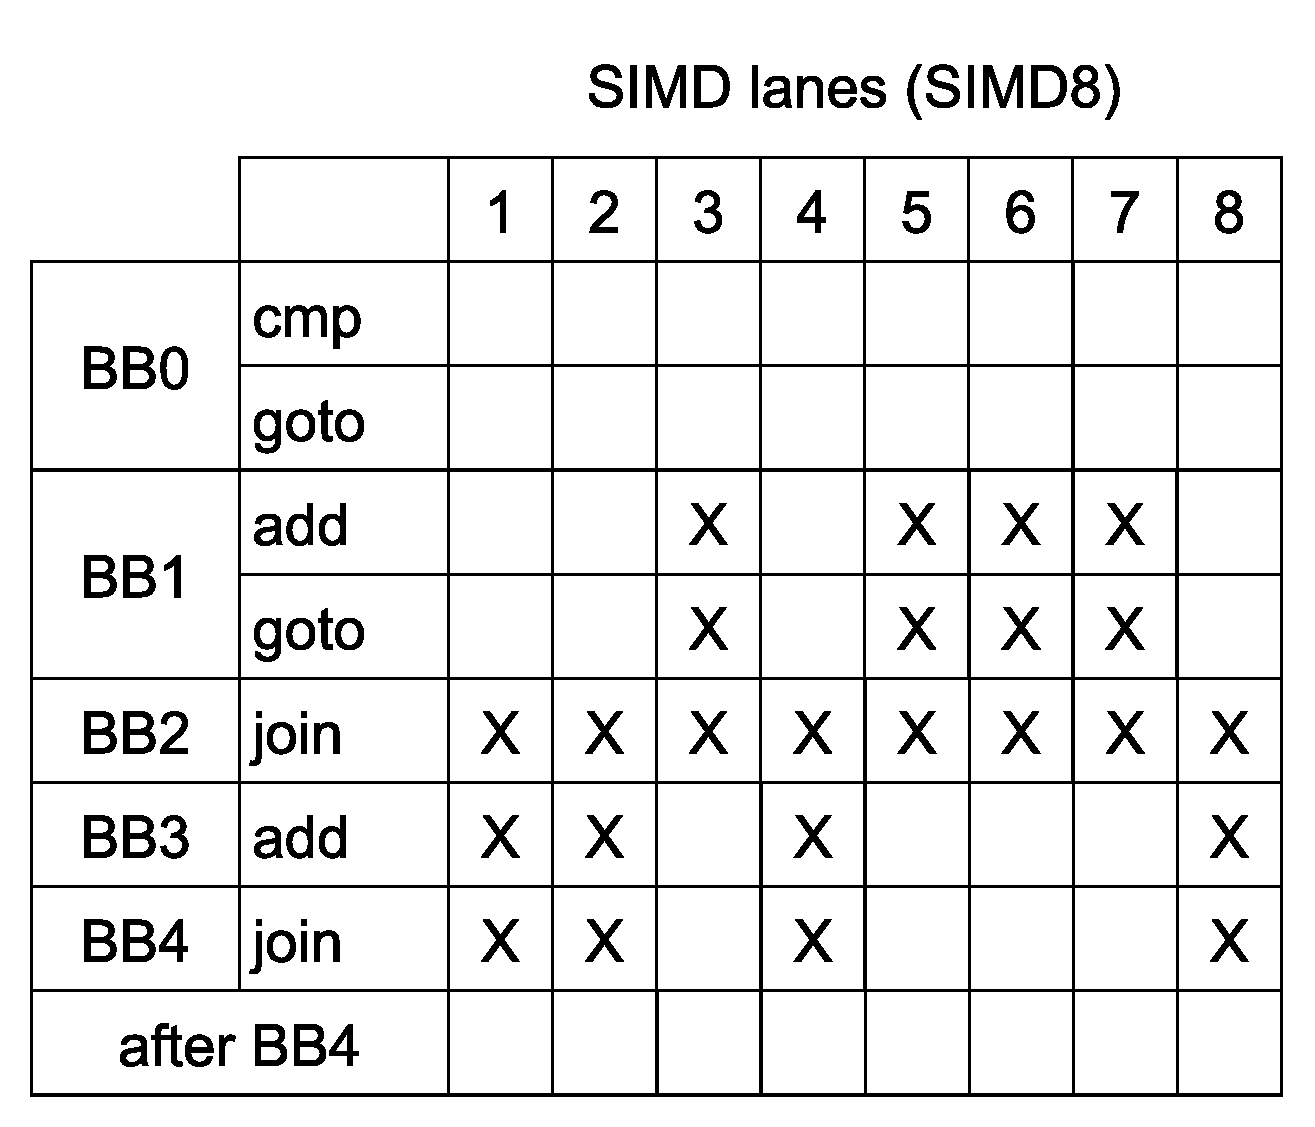
\includegraphics[scale=0.5]{Vladimirov/images/HW-goto-example.pdf}
    }
    \caption{Схема векторного потока управления}\label{fig:HW-goto-example}
\end{figure}

На рисунке~\ref{fig:HW-goto-example} схематично изображено, как будет происходить исполнение данного кода. Цифрами сверху обозначены номера линий исполнения в SIMD АЛУ, зеленым обозначены включенные линии, после исполнения предшествовавшей инструкции, а оранжевым -- выключенные.

\section{Обзор существующих подходов к векторизации}\label{sec:overview/vectorizing}

\subsection{Скалярная ISA и скалярное API}\label{subsec:overview/vectorizing/cuda}

Cuda, NVPTX. Гибкая векторизация за счёт механизмов HW. Сложное и дорогое железо.

\subsection{Векторная ISA и скалярное API}\label{subsec:overview/vectorizing/sycl}

OpenCL, SYCL. Векторизация после основных оптимизаций как часть кодогенерации. Проблемы с векторизацией внешних циклов. Необходимость SIMDX-dispatch, влияние на распределение регистров.

\subsection{Векторное API с ручным управлением регистровым файлом}\label{subsec:overview/vectorizing/cm}

CM. Минимальная роль компилятора. Крайне сложное программирование.

CM (C-for-Metal) -- язык программирования, являющийся расширением С++ и явно реализующий концепцию SIMD. CM является языком с раздельным исходным кодом, то есть компиляция кода хоста и кода устройства происходит раздельно. На данный момент целевыми являются только архитектуры графических ускорителей Intel.

Главной особенностью CM являются новые встроенные типы: \texttt{vector} (вектор), \texttt{vector\_ref} (ссылка на вектор), \texttt{matrix} (матрица) и \texttt{matrix\_ref} (ссылка на матрицу). Каждый из этих типов является шаблонным. Типы \texttt{vector} и \texttt{vector\_ref} имеют два шаблонных параметра: тип элемента и количество элементов. Типы \texttt{matrix} и \texttt{matrix\_ref} имеют три шаблонных
параметра: тип элемента, количество столбцов и количество строк матрицы. Типом элемента может быть любой примитивный целочисленный тип или тип числа с плавающей точкой

\section{Постановка задачи}\label{sec:overview/howtobetter}

Видно что никто не справляется. Надо сделать лучше.

\section{Выводы}\label{sec:overview/outcome}

В первой главе дается классификация

\FloatBarrier
